\begin{figure*}
	\begin{center}
	  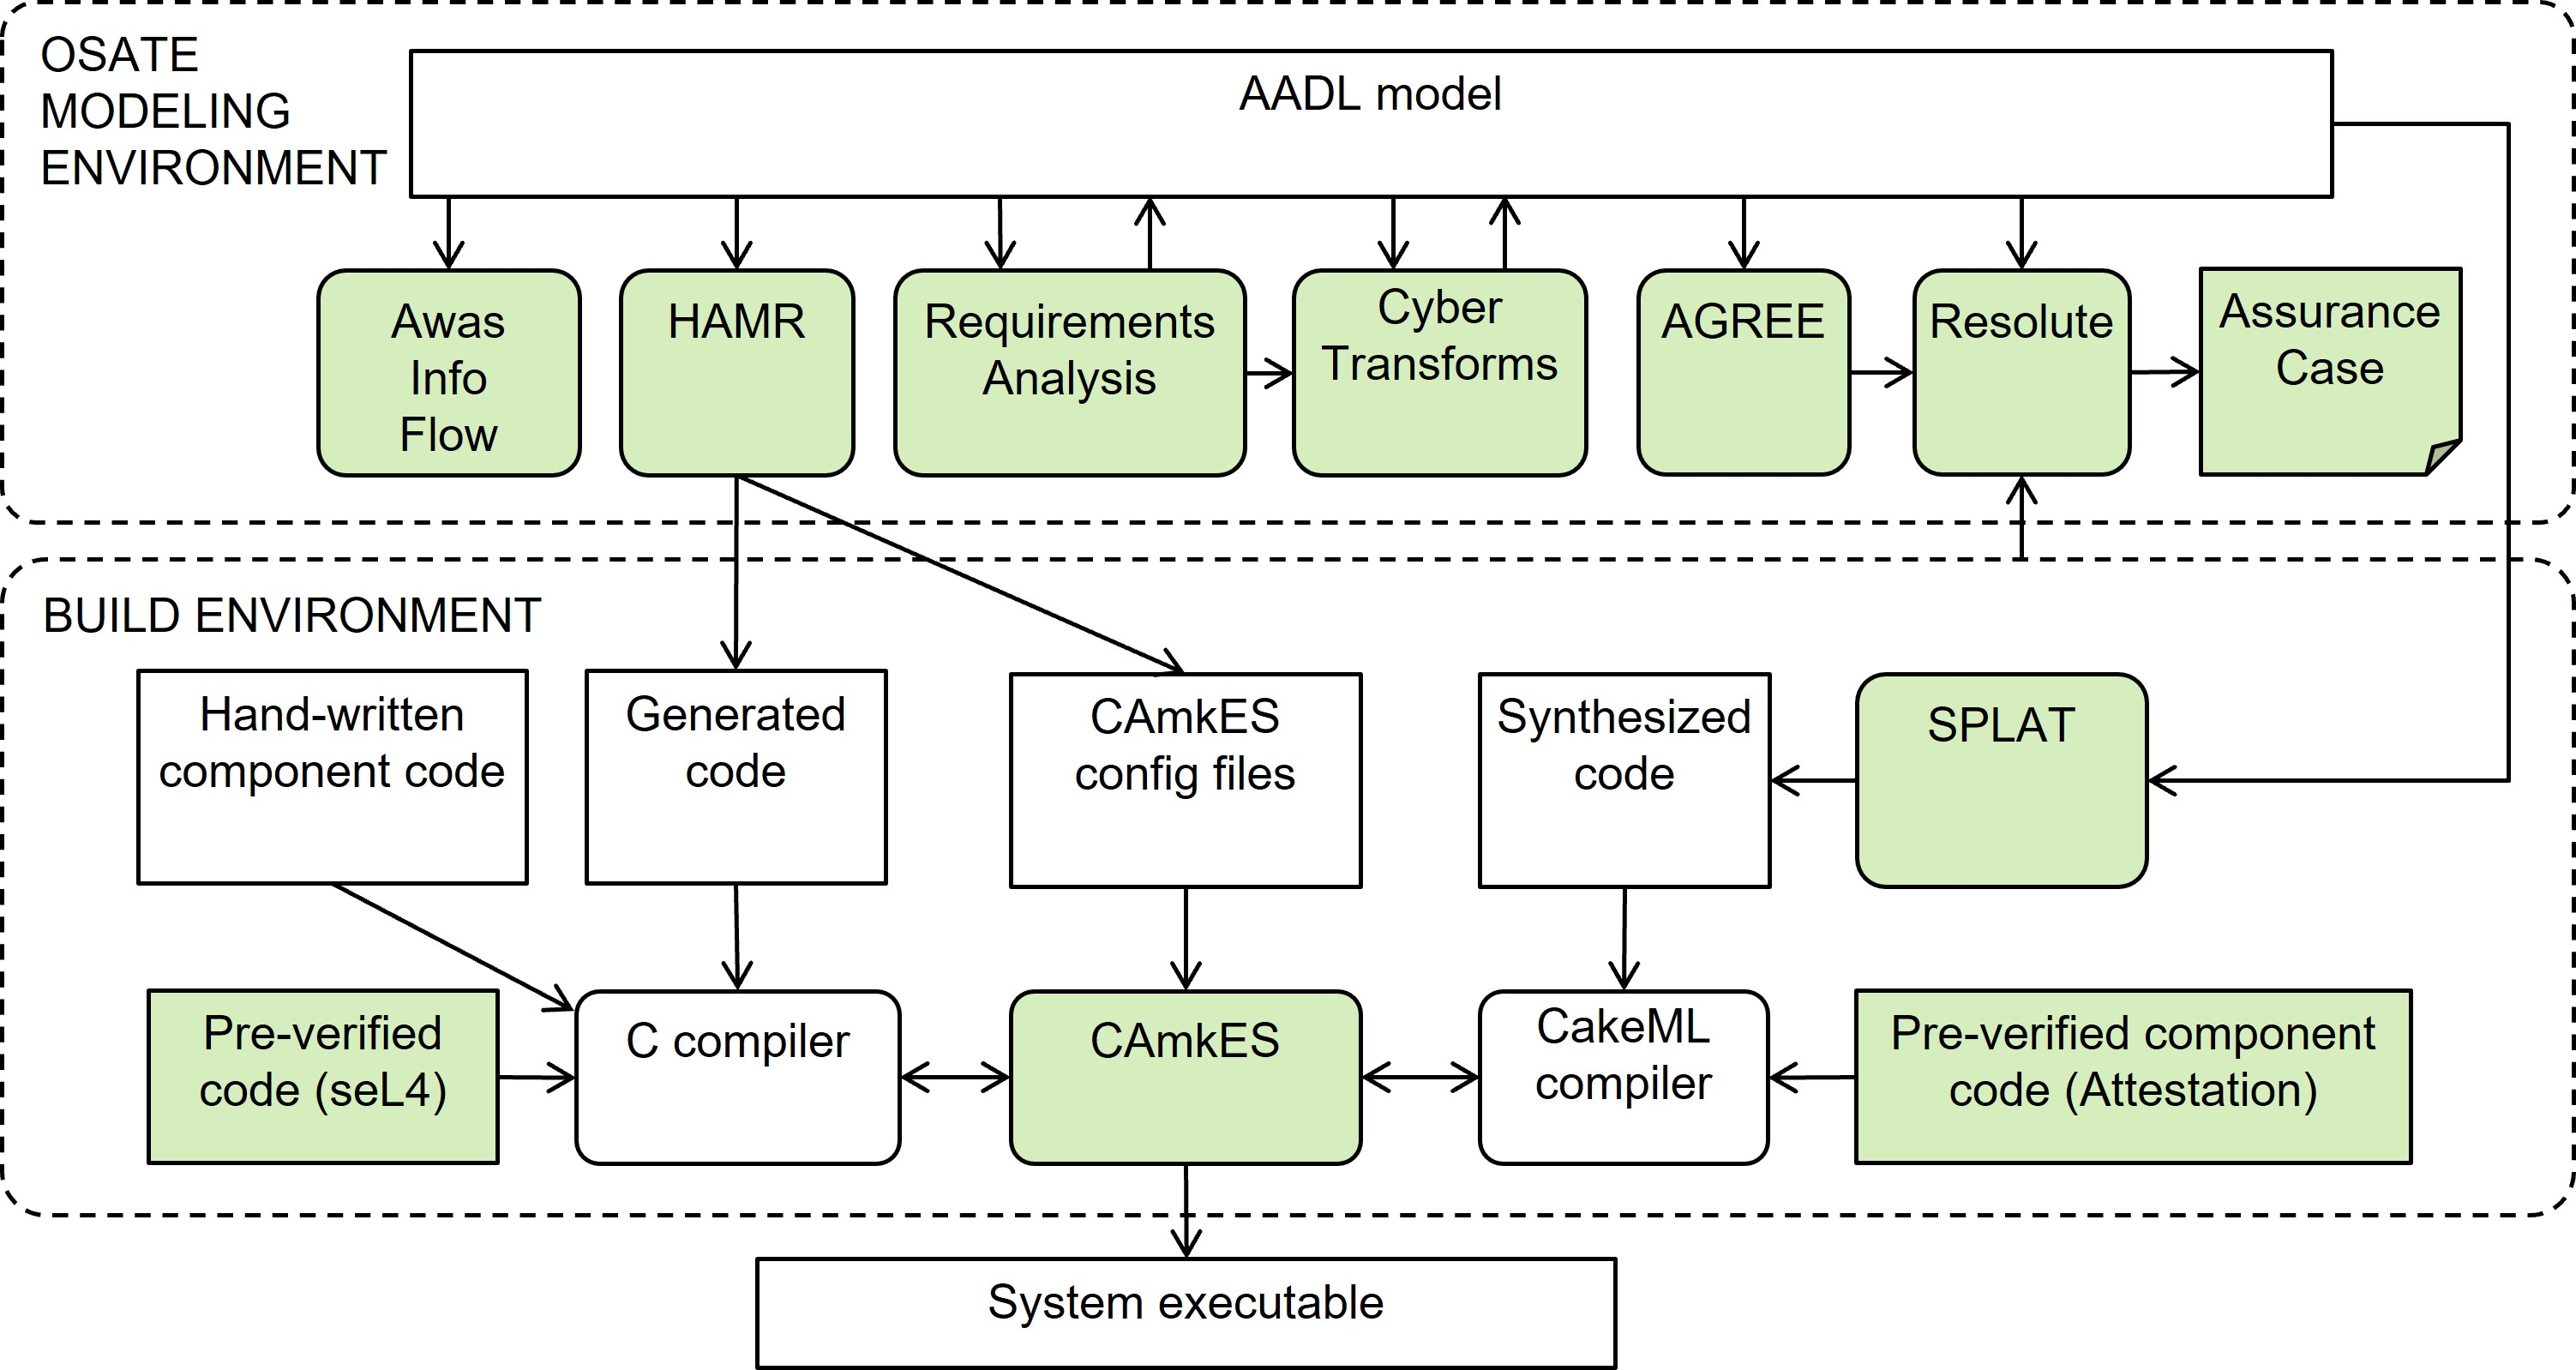
\includegraphics[width=\textwidth]{./figs/tool-arch.jpg}
  	\end{center}
	\caption{\brfcs\ integrated tool architecture with key components in the general workflow shown in green.} 
	\label{fig:tool-arch} 
\end{figure*}

The BriefCASE OSATE environment, \figref{fig:tool-arch}, provides designers with workflow and tool support for developing products with inherent cyber-resiliency.
It starts with the development of a baseline AADL model of the system architecture that defines the desired functionality.
This model can be evaluated using existing tools such as resource usage, information flow, latency analysis, etc. for validation.

\brfcs\ integrates additional tools into OSATE to analyze, identify, and address cybersecurity vulnerabilities in the baseline AADL model (top of \figref{fig:tool-arch}).
\brfcs\ provides access to analysis tools that examine the model, report potential cyber vulnerabilities,
and suggest requirements for mitigation \cite{dcrypps2019,gearcase2020}.
Designers add these requirements to the \brfcs\ project requirements repository. 
A key part of the requirements management in \brfcs\ is a corresponding assurance case that provides evidence, computed directly from the model or by supporting analysis tools, showing how each requirement is satisfied.
Evidential statements must exist to address the added cyber requirements in order for \brfcs\ to build the assurance case for the project.

\brfcs\ provides an extendable library of model transformations to address requirements for common cyber vulnerabilities:
\begin{compactitem}
	\item \textbf{Filter}: block messages that do not conform to a given specification
	\item \textbf{Monitor}: detect and alert violations at runtime
	\item \textbf{Gate}: block messages in the presence of an alert
	\item \textbf{Attestation}: measure non-local software to assess trustworthiness
	\item \textbf{Virtualization}: isolate components with virtualization
	\item \textbf{Proxy}: enable HTTPS message inspection 
	\item \textbf{seL4}: transform component definitions for the seL4 secure micro kernel
\end{compactitem}
Transformations update the AADL model architecture with new components and the assurance case with new required evidential statements.

Filters, monitors, and gates are considered high assurance components that require formal reasoning in building the assurance case.
When added to a system, \brfcs\ requires evidence that such components are 
\begin{compactenum}
	\item connected in the model, 
	\item cannot be bypassed, 
	\item meet their intended purposes, and
	\item are properly implemented.
\end{compactenum}
Information flow analysis provides evidence for the first two properties while model checking and code synthesis provide evidence for the last two properties.

The Awas AADL information flow analyzer and visualizer provides evidence that high assurance components are connected and not bypassed in the model \cite{awas}.
The High Assurance Modeling and Rapid engineering for embedded systems tool (HAMR) generates from the model component infrastructure and integration code implementing the semantics of AADL-compliant thread scheduling, thread dispatching, port-based communication, and real-time scheduling \cite{hamr}.
Along with that code generation, HAMR constructs a proof that all flows in the AADL model are in the implementation and that no extraneous flows have been added to the implementation.
HAMR relies on the seL4 microkernel for its proofs.
The seL4 microkernel, among other security properties, provides strong isolation between components ensuring that there are no communication channels outside of what is defined \cite{sel4-sosp09, sel4-tocs14, sel4-cacm18}.

The Assume Guarantee Reasoning Environment (AGREE) is a compositional, assume-guarantee-style, model checker for AADL models \cite{compositional-analysis-agree,nfm:agree}. 
AGREE attempts to prove properties about one layer of the architecture using properties allocated to sub-components.
The composition is performed in terms of \emph{contracts} provided for each component and sub-component that state \emph{assumptions} on inputs and \emph{guarantees} on outputs under the assumptions.
AGREE verifies the \emph{consistency} of the composition of the component and sub-component contracts meaning that in every connection the source constraints satisfy the destination constraints.

The contributions discussed in this manuscript relate to the aspects of \brfcs\ concerning evidence that a high-assurance component meets its intended purpose and is properly implemented.
This manuscript defines a \emph{code contract} language that is a subset of the AGREE language with sequential evaluation semantics as opposed to the existing parallel semantics of AGREE.
The sequential semantics are requisite to code synthesis and are defined such that AGREE is able to still prove consistency in the contract composition of the model. 
As such, the behavior of a high assurance component is defined by the designer in a code contract, and AGREE proves that the code contract meets its intended purpose in two ways: first, its input to output definition is satisfied, and second, in the system composition, it satisfies associated cyber-requirements.

Showing that a component is properly implemented is accomplished through formal synthesis from the code contract.
The Semantic Properties of Language and Automata Theory (SPLAT) tool generates \emph{CakeML} code to implement the code contract.
The CakeML compiler is verified to generate binary implementations that are equivalent in semantics to the original input program \cite{cakeml}.
It proves that the resulting binary exactly preserves the meaning of the original contract to assure that the component is properly implemented.